\documentclass[conference]{IEEEtran}
\IEEEoverridecommandlockouts
% The preceding line is only needed to identify funding in the first footnote. If that is unneeded, please comment it out.
\usepackage{cite}
\usepackage{amsmath,amssymb,amsfonts}
\usepackage{algorithmic}
\usepackage{graphicx}
\usepackage{textcomp}
\usepackage{multirow}
\usepackage{xcolor}
\usepackage[hyphens]{url} % defines \url
\urlstyle{same}
\def\BibTeX{{\rm B\kern-.05em{\sc i\kern-.025em b}\kern-.08em
    T\kern-.1667em\lower.7ex\hbox{E}\kern-.125emX}}
\begin{document}

\title{Benchmarking and Evaluating Time Series Databases for Appliance-Level Energy Consumption Data\\
}

\author{\IEEEauthorblockN{Simin Shehbaz}
\IEEEauthorblockA{\textit{Faculty of Computer Science} \\
\textit{University of New Brunswick}\\
Fredericton, Canada \\
simin.shehbaz@unb.ca}
\and
\IEEEauthorblockN{Mohammad Mehabadi}
\IEEEauthorblockA{\textit{Faculty of Computer Science} \\
\textit{University of New Brunswick}\\
Fredericton, Canada \\
m.mehabadi@unb.ca}
\and
\IEEEauthorblockN{Kenneth B. Kent}
\IEEEauthorblockA{\textit{Faculty of Computer Science} \\
\textit{University of New Brunswick}\\
Fredericton, Canada \\
ken@unb.ca}
}

\maketitle

\begin{abstract}
Time series databases (TSDBs) are widely used to store high-frequency energy consumption data, but their performance varies depending on workload characteristics. This paper benchmarks leading TSDBs to identify their suitability to handle appliance-level, per-minute energy data. While prior work has evaluated TSDBs, limited research has been done on TSDBs for wide-format, fine-grained residential energy data at the appliance level. We introduce a custom-generated dataset simulating the usage of twenty-six appliances across five household types in a wide-format schema. Building on the TSM-Bench framework, we adapt it to support our appliance-level dataset, domain-specific workloads, and evaluation metrics. We analyze ingestion and query performance across three TSDBs that support this wide-format, while highlighting the trade-offs in latency, resource usage, throughput and storage.

Looking ahead, we plan to evaluate schema transformations (wide to narrow), explore additional TSDBs optimized for narrow-format ingestion and compare their performance against wide-format results. These measures aim to provide a comprehensive and  format-aware comparison of TSDBs.
\end{abstract}

\begin{IEEEkeywords}
time series databases, benchmarking, IoT, energy consumption, benchmark workloads, ingestion \& query performance
\end{IEEEkeywords}

\section{Introduction}
The rise of smart homes, Internet of Things (IoT)-enabled devices, and renewable energy systems have made \textbf{appliance-level energy consumption data} a critical resource for building intelligent infrastructure. Capturing this data at a \textbf{minute-level frequency} from dozens of appliances produces large-scale, multi-dimensional time series data—demanding efficient storage, querying, and analysis. Time series databases (TSDBs) are essential for managing large volumes of time-stamped data with \textbf{low-latency read and write performance}. They are preferred over general-purpose databases in real-time monitoring applications, due to their \textbf{scalability, compression efficiency}, and native support for \textbf{streaming analytics}~\cite{1_tsmbench2023}. TSDBs use time-based indexing, columnar storage, downsampling strategies, and offer built-in support for temporal queries such as sliding windows, aggregations, and time filters~\cite{1_tsmbench2023}.  Unlike traditional relational databases, TSDBs are optimized for \textbf{high ingestion throughput} and storage efficiency~\cite{1_tsmbench2023,2_tsmsurvey2017}. 

A crucial design choice when storing time series data is the schema format—wide vs. narrow. In the \textbf{wide format}, each row contains multiple sensor readings for a single timestamp. In contrast, the \textbf{narrow format} stores one measurement per row, requiring additional columns for the sensor identifier and its value. Wide-format schemas are typically better suited for high-dimensional sensor data where all sensors report at the same interval, enabling faster cross-sensor operations and improved compression due to columnar locality~\cite{6_clickbench}. However, they may be less flexible for variable-frequency streams or semi-structured data, where narrow formats are more common~\cite{2_tsmsurvey2017}.

In the context of the appliance-level energy data that we are addressing in this paper, typical analyses on this data would include: \textbf{trends over time} (e.g., how the heater consumption varies seasonally), \textbf{anomaly detection} that identifies surges in energy readings (e.g., devices left on), \textbf{device-level usage comparison}, and checking for \textbf{peak demands}, showing the critical role of TSDBs in analytics. 

Existing benchmarks have not evaluated systems under appliance-level energy workloads. They have focused on specific domains like financial transactions, smart buildings, and industrial instruments~\cite{3_tsbs,4_smartbench2020,5_scits2022}. TSM-Bench comes close in scope, and caters to wide-formatted data~\cite{1_tsmbench2023}. Hence we extend this framework, tailoring it to our fine-grained, appliance-level, energy dataset that exhibits: high dimensionality, wide-format rows, frequent data points (minute-level), and realistic workloads.

Every testing system is optimized around trade-offs made in storage formatting, indexing, compression and query execution~\cite{1_tsmbench2023,2_tsmsurvey2017,6_clickbench}. Therefore, this work presents a comprehensive benchmarking framework for appliance-level energy data that extends the TSM-Bench, while making the following contributions:
\begin{itemize}
  \item Developing a benchmarking framework tailored to appliance-level energy consumption, evaluating both ingestion and query performance.
  \item Generating data workloads using \textbf{`DGSim'}, a custom simulator that simulates realistic energy consumption patterns for 26 appliances across five household types, producing wide-format, minute-level time series data~\cite{17_DGSim}.
  \item Defining a varying set of workload strains including write-heavy streams, range queries, time aggregations (daily/monthly), and appliance-level comparisons.
  \item Benchmarking three leading TSDBs: TimescaleDB, QuestDB and ClickHouse.
\end{itemize}

The remainder of the paper is structured as follows: Section~\ref{sec:related} reviews related work on TSDB benchmarking and appliance-level datasets. Section~\ref{sec:setup} presents the study setup, Section~\ref{sec:framework} details the benchmarking framework. Section~\ref{sec:results} reports and analyzes the experimental results. Section~\ref{sec:conclusion} concludes the paper, and Section~\ref{sec:future} outlines future research directions.


\section{Related Work}\label{sec:related}
Numerous benchmarks have been proposed to evaluate TSDBs, each tailored to specific application domains and workload characteristics.

\textbf{TSM-Bench} is among the most comprehensive benchmarks for TSDBs used in monitoring environments~\cite{1_tsmbench2023}. It introduces offline and online workload tiers, a suite of fundamental time-based queries, and a novel Generative Adversarial Network (GAN)-based data generator (TS-LSH) tailored specifically for hydrological data. While powerful, its design is domain-specific and does not generalize well to energy datasets. Time Series Benchmark Suite (\textbf{TSBS}) is widely used in industry to compare storage size, loading time, and aggregation performance across systems like InfluxDB and TimescaleDB~\cite{3_tsbs}. However, TSBS is heavily geared toward finance and DevOps metrics, and lacks native support for wide-format ingestion and complex device-level analytics~\cite{3_tsbs}.
\textbf{SciTS} benchmarks TSDBs for scientific instrumentation use cases. It uses synthetic data to evaluate ingestion and query latency~\cite{5_scits2022}. SmartBench evaluates data systems for smart buildings~\cite{4_smartbench2020}. However, it limits its scope to correlation queries and basic filtering on noisy datasets. 
\textbf{IoTDB-Benchmark} focuses on heterogeneous IoT data with different sensor types and frequencies~\cite{7_iotdbbenchmark}. It evaluates ingestion throughput and query performance but assumes narrow-format, homogeneous time series and does not support appliance-level complexity.
\textbf{IoTAbench} was proposed as a benchmark for IoT analytics platforms and uses real-world sensor data to assess ingestion and analytics performance~\cite{9_iotabench2015}. While highlighting power usage scenarios, it uses simplified event models and focuses on system-level throughput over schema variations.
\textbf{TS-Benchmark} is tailored to benchmark electricity data from wind turbines, while incorporating realistic workloads including anomaly detection and multi-sensor fetches. However, it is limited to offline evaluation and assumes a relatively simple data layout patterns~\cite{10_tsbenchmark2021}.
An important system-level study is the encoding analysis for \textbf{Apache IoTDB}, which compares time series compression formats under various characteristics including data repetition, sparsity, and delta distribution~\cite{11_iotdbencoding2022}.

Collectively, these benchmarks have advanced TSDB evaluation. However, none offer an end-to-end assessment for appliance-level energy data, which requires support for wide and narrow schema comparisons, multi-sensor queries, and concurrent streaming and analytics—core demands in smart energy systems.


\section{Experimental Setup}\label{sec:setup}
This section outlines the data generation process, data characteristics, and the process of selecting TSDBs that are used in this study.
\subsection{Data Generation}
The dataset used in this study is generated using \textbf{`DGSim'}, developed in prior work under this study~\cite{17_DGSim}. This models appliance-level energy consumption based on the usage patterns of various household appliances. It has been designed to model realistic energy consumption patterns by appliances including those of heating, ventilation, and air conditioning (HVAC) systems, refrigerators, and washing machines. DGSim adopts a \textbf{Markov, state-based modeling technique}, where each appliance is modeled as a probabilistic state machine~\cite{12_zucchini2016hmm}. This simulator provides a scalable, reproducible environment for generating data as required by the experiment. 
DGSim originally generated aggregated energy consumption profiles for a large number of households. For the purpose of this benchmarking study, the simulator was modified to output disaggregated, appliance-level energy consumption data for individual households.

\subsection{Data Characteristics}
The generated dataset follows a wide format, where each row represents a timestamp and each column corresponds to a specific appliance. It captures minute-level energy consumption for twenty-six appliances over a user-defined time range. DGSim supports five distinct household types: single-family attached, single-family detached, mobile home, two-to-four room apartment and apartments with more than five rooms. Each of these have different consumption patterns.
For this study, datasets were exported as CSV files prior to ingestion. Table~\ref{tab:dataset_characteristics} summarizes the structure and attributes of the appliance-level energy consumption dataset.

\begin{table}[tb]
\caption{Characteristics of the Energy Consumption Dataset}
\begin{center}
    \renewcommand{\arraystretch}{1.15}
\begin{tabular}{|l|l|}
\hline
\textbf{Characteristic} & \textbf{Description} \\
\hline
Time Granularity & 1-minute \\
Time Range & User-specified (day, month, year) \\
Appliances Modeled & 26 \\
Number of Columns & 30 \\
Dataset Format & Wide (one column per appliance) \\
House Types & 5 distinct types \\
Operations & Simulate → Insert → Query \\
Storage Format & CSV (pre-ingestion), TSDB (post-ingestion) \\
\hline
\end{tabular}
\label{tab:dataset_characteristics}
\end{center}
\end{table}

\subsection{TSDBs' Inclusion and Exclusion Criteria}
We have defined a set of inclusion and exclusion criteria to select the appropriate TSDBs for this benchmarking study. The criteria are as follows:
\subsubsection{Inclusion Criteria}
\begin{itemize}
    \item Native support for time-series data, indexing, and storage
    \item Open-source or free for academic use
    \item Ability to ingest wide and narrow format data
    \item Support for time-based queries, filtering, and aggregation
    \item Native support for Docker-based deployment
\end{itemize}
\subsubsection{Exclusion Criteria}
\begin{itemize}
    \item Unmaintained or inactive projects, or projects that have had no updates in over a year
\end{itemize}

\subsection{Selected TSDBs for Benchmark Study}
Starting with a list of thirty-one TSDBs identified through literature and community sources, we applied the above criteria to narrow the selection to four candidates.
ClickHouse is a high-performance columnar database with strong support for wide schemas. Its \textbf{MergeTree} engine enables high ingestion rates through \textbf{delta encoding} and \textbf{Single Instruction Multiple Data (SIMD)-optimized scans}~\cite{6_clickbench}.
TimescaleDB, built on PostgreSQL, stores time series data in row-oriented \textbf{hyper-tables}, partitioned by time. It handles wide rows effectively by using array-based storage and \textbf{chunk-level compression}~\cite{2_tsmsurvey2017}.
 QuestDB is a lightweight TSDB using column-store layout with time-partitioned tables and \textbf{memory-mapped I/O}. It supports wide schemas but lacks advanced compression, leading to a larger storage footprint~\cite{13_questdbdocs}.
Although flexible and JSON-friendly, CrateDB has an inverted index structure and is inefficient for wide-schema ingestion with frequent updates~\cite{15_rinaldi2019}. During preliminary testing, it showed significant bottlenecks, and was excluded from comparative analysis.
The final TSDBs selected were: \textbf{TimescaleDB}, \textbf{QuestDB}, and \textbf{ClickHouse}.

\section{Benchmarking Framework}\label{sec:framework}

This benchmarking framework is based on the TSM Benchmarking framework~\cite{1_tsmbench2023}, which is a widely used benchmarking framework for TSDBs.  Modifications were made to extend TSM-Bench, to accommodate the specific requirements of this study, such as the data generation process, the selected TSDBs, the queries to be executed, and the performance metrics to be measured for the write and read testing. This allowed testing TSDBs' performances under realistic conditions derived from a well-defined, minute and appliance-level energy dataset.

\subsection{Pre-Defined Workload Configurations}
To evaluate TSDB performance under varying load conditions, we define five scalable workload tiers (W1–-W5). Each workload is generated using DGSim with the same schema and structure, but differs in scale (e.g., number of households, duration, and data volume). Prior to ingestion, a lightweight lossy compression step is applied to the dataset: all numerical values are rounded to two decimal places to reduce precision without affecting benchmark integrity. Aside from this, the datasets remain unchanged.

As summarized in Table~\ref{tab:workload_configurations}, W1--W5 simulates appliance level household energy usage, with all datasets recorded at a one-minute interval for twenty-six appliances per house. The data points are represented in millions (M) as shown in Table~\ref{tab:workload_configurations}. All workloads comprise of thirty columns, having the same characteristics as shown in Table~\ref{tab:dataset_characteristics}. W1 represents a baseline ingestion test with minimal load, while W5 simulates a high stress scenario involving over 44 million rows and 1.3 billion data points.
\begin{table}[tbp]
\caption{Workload Tiers}
\begin{center}
\renewcommand{\arraystretch}{1.4}
\begin{tabular}{|c|c|c|c|c|c|c|}
    \hline
    \textbf{Duration} & \textbf{ID} & \textbf{Houses} & \textbf{Data Points (M)} & \textbf{Rows} & \textbf{Size (GB)} \\
    \hline
    \multirow{3}{*}{\shortstack{1 Day}} 
        & W1 & 100   & 4.32   & 144,000     & 0.0287 \\
        & W2 & 1,000 & 43.20  & 1,440,000   & 0.289 \\
        & W3 & 5,000 & 216.00 & 7,200,000   & 1.450 \\
    \hline
    \multirow{2}{*}{\shortstack{1 Month}} 
        & W4 & 100   & 133.80 & 4,464,000   & 0.898 \\
        & W5 & 1,000 & 1338.00& 44,640,000  & 9.04 \\
    \hline
\end{tabular}
\label{tab:workload_configurations}
\end{center}
\end{table}

\subsection{Ingestion Workload Design}
Ingestion performance is evaluated across all five workloads (W1–W5), as outlined in Table~\ref{tab:workload_configurations}. Each ingestion test involves loading the entire dataset in bulk, simulating real-world scenarios where historical energy data is inserted in batches. The following metrics are recorded:
\begin{itemize}
  \item \textbf{Ingestion latency}: The total time taken to ingest the
entire dataset for a workload tier.
  \item \textbf{Ingestion Throughput}: Calculated as rows inserted per second providing a measure of how quickly the database can handle incoming data.
  \item \textbf{Storage Size}: The total disk space used by the database
after ingestion.
\end{itemize}

\subsection{Query Workload Design}
In our application domain, the query workload is structured to test the TSDBs' ability to handle common time-series access patterns, such as consumption queries, detect threshold violations, usage summaries, compare appliance behaviors, and perform aggregations.
As a result, the queries have been divided into two main categories: \textbf{point queries} and \textbf{analytical queries}. Point queries are designed to retrieve specific data points, while analytical queries are designed to perform aggregations and calculations on the data. This structure follows the precedent set by pre-existing benchmarks, which advocate for a mix of point queries, aggregations, and downsampling to evaluate TSDB capabilities comprehensively~\cite{3_tsbs,11_iotdbencoding2022}.
\subsubsection{Point Queries}
The point queries used in this study are:
\begin{itemize}
    \item \textbf{Q1--Data Fetching}: Retrieve the minute-level peak energy consumption for all appliances during peak usage hours.
    \item \textbf{Q2--Data Fetching with Filters}: Retrieve the minute-level energy consumption for a specific appliance, filtering where the consumption exceeds a defined threshold.
\end{itemize}
\subsubsection{Analytical Queries}
Analytical queries are designed to typically summarize data over a specific time range, or to perform calculations on the data. The analytical queries used in this study are:
\begin{itemize}
  \item \textbf{Q3--Cross-Appliance Average}: Computes average values across two or more appliances for a single household. 
  \item \textbf{Q4--Average Energy Consumption by House Type}: Computes the average total energy consumption grouped by house type.   
  \item \textbf{Q5--Average Energy Consumption by House}: Computes the average energy consumption per household.      
  \item \textbf{Q6--Hourly Downsampling}: Aggregates minute-level readings into hourly averages for each appliance and household.     
\end{itemize}

For query performance evaluation, we use only the largest workload (W5). Since all workloads share the same core structure, this approach avoids redundancy while ensuring a high-stress and representative query environment. The results are averaged over three runs for each query type. This test measures the query latency, throughput, result size, CPU usage, and memory consumption for each query type across the selected TSDBs.

\subsection{Hardware Setup Notes}
To ensure consistency, all TSDBs are deployed in isolated docker containers with identical hardware configurations, on a local machine. Docker was chosen due to its ability to provide isolated and consistent testing environments across the databases, hence eliminating system-level dependencies that may affect performance results~\cite{16_felter2015docker}. 
Each database container was initialized using default configuration parameters, unless otherwise required by the database. The following specifications were used for the benchmarking tests:
\begin{itemize}
  \item \textbf{Host Machine}: Apple M1 Pro, 10 CPU cores, 32GB
  \item \textbf{Docker Version}: v28.1.1, build 4eba377
  \item \textbf{TimescaleDB}: v2.19.3 (PostgreSQL 14.17)
  \item \textbf{QuestDB}: v7.3.2
  \item \textbf{ClickHouse}: v25.5.2.47
\end{itemize}

Docker images were pinned to specific, ARM64-stable versions to ensure reproducibility on Apple M1 hardware and to avoid confounding our results with evolving optimizer and storage changes. These versions fully support the features required by our workloads.

Each test undergoes an initial warm-up run, followed by three measured runs to capture performance. TSDBs are reset between each run. This methodology ensures a fair, controlled, and reproducible comparison of read and write performance across systems.

\section{Results And Analysis}\label{sec:results}
This section presents the results of the benchmarking experiments conducted on the selected TSDBs using both ingestion and query workloads.

\subsection{Ingestion Results}
In this section, we evaluate the ingestion performance of \textbf{TimescaleDB}, \textbf{QuestDB}, and \textbf{ClickHouse} across five workload tiers (W1--W5). These reflect increasing volumes of appliance-level energy consumption data. The results are discussed in the following subsections.

\subsubsection{Ingestion Latency}
Fig.~\ref{fig:ingestion_latency_comparison} illustrates the ingestion latency for each TSDB across the five workload tiers. The results show that \textbf{ClickHouse consistently outperforms} both TimescaleDB and QuestDB in terms of ingestion latency, particularly for larger workloads. This trend is consistent across all workloads. The ingestion latency of TimescaleDB increased significantly beyond W3, likely due to hyper-table chunk management and background compression tasks.
\begin{figure}[tb]
\centering
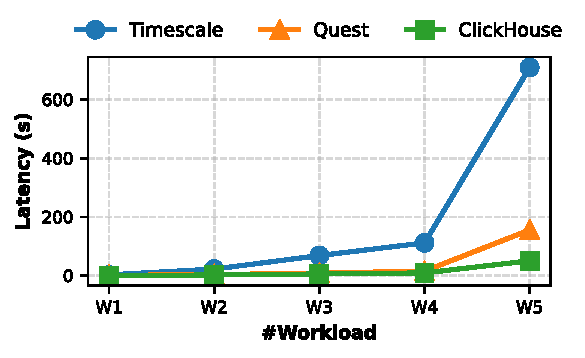
\includegraphics[width=0.9\linewidth]{1_ing_latency_plot.pdf}
\caption{Ingestion latency comparison across TSDBs for Each Workload.}
\label{fig:ingestion_latency_comparison}
\end{figure}

\subsubsection{Ingestion Throughput}
Fig.~\ref{fig:ingestion_throughput_comparison} shows that ClickHouse performs the best. On W5, \textbf{ClickHouse achieved the highest throughput} at 891K rows/sec, followed by QuestDB at 287K rows/sec. TimescaleDB showed a consistent but relatively low throughput. QuestDB showed reduced performance on larger workloads.
\begin{figure}[tb]
\centering
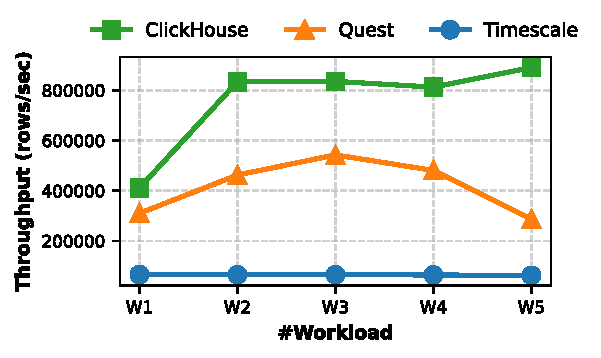
\includegraphics[width=0.8\linewidth]{2_ing_throughput_plot.pdf}
\caption{Ingestion throughput comparison across TSDBs for Each Workload.}
\label{fig:ingestion_throughput_comparison}
\end{figure}

\subsubsection{Ingestion Storage Footprint}
Fig.~\ref{fig:ingestion_storage_comparison} illustrates the storage size used by each TSDB after ingesting the datasets for each workload tier. Looking at only the standard storage, we observe that all the databases use up more space than the original CSV file. Among the TSDBs, \textbf{ClickHouse shows the lowest storage footprint} across all workloads. Post compression, ClickHouse achieves the best storage. Its storage footprint is significantly reduced when compared to the original CSV file. QuestDB does not apply compression, and therefore, its storage size remains constant across all workloads. Compression in TimescaleDB does show a decrease in storage size, performing better than QuestDB in terms of storage efficiency.
\begin{figure}[tb]
\centering
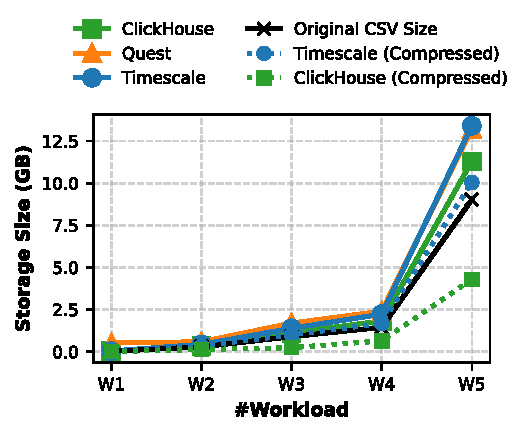
\includegraphics[width=0.8\linewidth]{3_ing_storage_plot.pdf}
\caption{Ingestion Storage Comparison Across TSDBs for Each Workload.}
\label{fig:ingestion_storage_comparison}
\end{figure}

\subsection{Query Results}
We benchmarked six queries (Q1-Q6) on W5 that are representative of common time series operations on appliance level energy consumption data. The results are summarized in Fig.~\ref{fig:query_latency_comparison}, Fig.~\ref{fig:query_memory_comparison} and Fig.~\ref{fig:query_cpu_comparison}.

\begin{figure}[tb]
\centering
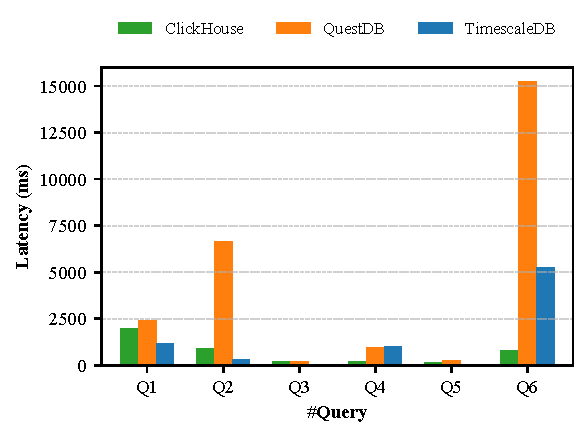
\includegraphics[width=0.8\linewidth]{1_query_latency_ieee.pdf}
\caption{Query Latency Comparison Across TSDBs.}
\label{fig:query_latency_comparison}
\end{figure}

\begin{figure}[tb]
\centering
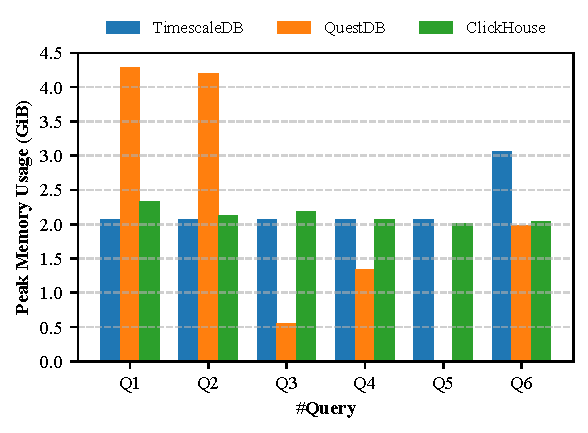
\includegraphics[width=0.8\linewidth]{2_query_memory.pdf}
\caption{Query Memory Usage Comparison Across TSDBs.}
\label{fig:query_memory_comparison}
\end{figure}

\begin{figure}[tb]
\centering
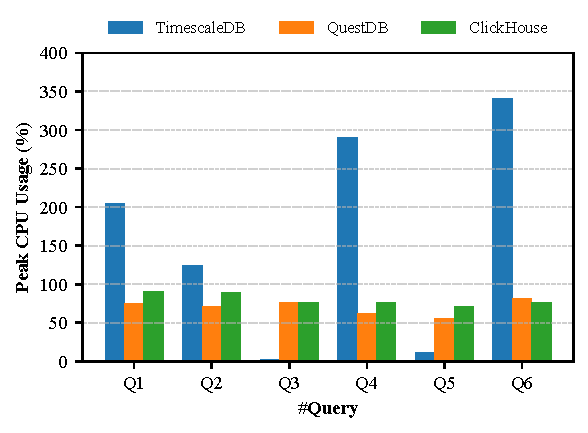
\includegraphics[width=0.8\linewidth]{3_query_cpu.pdf}
\caption{Query CPU Usage Comparison Across TSDBs.}
\label{fig:query_cpu_comparison}
\end{figure}

\subsubsection{Q1}
TimescaleDB performs well on simple data retrieval due to hyper-table chunking and time-based pruning. However, CPU spikes (204\%) suggest that internal decompression or indexing is resource-intensive.
QuestDB performs the worst. Despite storing data in time-partitioned files, it scans extra data due to a lack of indexing granularity and full-column reads.
ClickHouse performs well. Its granule-level access reduces IO, but its MergeTree parts are not helpful here since they are optimized for large batch reads, not point lookups.

\subsubsection{Q2}

Although TimescaleDB is quick, its filtered queries are computationally heavier since it needs to read and decompress chunks, and apply filters post-decompression, resulting in a higher CPU usage (124\%).
QuestDB's Performance is poor. It materializes full rows before applying filters, and lacks indexed predicate push-down.
ClickHouse performs reasonably well. The combination of sparse indexing and vectorized filtering using SIMD instructions makes it ideal for appliance anomaly detection or high-frequency filter queries.

\subsubsection{Q3}
Here, TimescaleDB is highly efficient (23 ms). Its array-based columnar chunks enable fast aggregation across appliance columns, and operates efficiently on grouped data.
QuestDB is decently optimized for per-row aggregation (190 ms), but not as fast as TimescaleDB\@. It stores data in columnar format but requires manual aggregation over many rows, which limits speed.
Since ClickHouse is a column-store, it does well with this query.

\subsubsection{Q4}
TimescaleDB's performance drops here due to multiple GROUP BY clauses across a large dataset. Decompression and re-aggregation across many house types cause high CPU usage and latency, revealing limits in chunk-level parallelism.
QuestDB has a high latency (938 ms) despite a reduced query scope suggests it struggles with multiple group-by operations. Its row-store access patterns require large in-memory scans.
ClickHouse has efficient aggregation engine groups and computes millions of rows in a few hundred ms. MergeTree partitions and parallel aggregation kernels accelerate time-based group-bys.

\subsubsection{Q5}

For TimescaleDB, although conceptually similar to Q4, Q5 involves fewer groupings and yields better performance (33 ms). Chunk pruning helps here reducing CPU usage.
This query runs reasonably (233 ms) for QuestDB, with fewer groupings and shorter ranges, benefitting from file-mapped IO for reading recent rows efficiently.
ClickHouse matches its performance on Q4. The system is efficient with group-by operations on high-cardinality columns like house IDs.

\subsubsection{Q6}
For TimescaleDB, resampling high-frequency data into hourly buckets across appliances is compute-heavy. This reflects challenges in chunk scan and aggregations under a compressed format.
For QuestDB, this is the weakest point (over 15 seconds). It lacks efficient windowed time grouping and processes the raw data sequentially, causing massive slowdowns.
ClickHouse is the best performer here (773 ms). It excels at SAMPLE BY and time-bucketing, applying parallel aggregation over time blocks with minimal memory overhead.

\section{Conclusion}\label{sec:conclusion}
This study evaluates the performance of three leading TSDBs—\textbf{TimescaleDB, QuestDB, and ClickHouse}—using a realistic, appliance-level energy dataset generated via DGSim. By extending the \textbf{TSM-Bench framework}, we benchmark ingestion and query performance across five workload tiers and six representative queries. ClickHouse consistently delivers the best overall performance, with the lowest ingestion latency, highest throughput, and most efficient compression. It also excels in complex analytical queries. TimescaleDB achieves the lowest latency for simple and grouped queries, but incurs higher CPU and memory costs for large-scale downsampling and compression. QuestDB, while lightweight and easy to deploy, shows limitations in indexing, making it less suitable for high-resolution, appliance-level workloads. Overall, we find \textbf{ClickHouse to be the most suitable TSDB} for appliance-level smart energy applications, offering the best trade-off between performance, efficiency, and query flexibility.

\section{Future Work}\label{sec:future}
Based on the insights garnered from this benchmarking study, we aim to explore three key areas to better analyze TSDBs for appliance-level energy data. 
First, investigating system-level optimization strategies within each TSDB, focusing on improving the read performance by possibly tuning indexing schemes, compression techniques, and partitioning policies. 
Next, we would like to explore the impact of converting the dataset from its current wide format, to a narrow format, and observe how that affects TSDB performance. Many TSDBs are specifically optimized for narrow schemas and often achieve better storage and ingestion performance under such conditions. Evaluating this conversion will help in understanding how schema structure influences compatibility, data efficiency, and execution performance across systems.
Linked to the previous point, we also plan to expand the scope of our study to include additional TSDBs that rely on narrow-format ingestion and alternative architectural models, including InfluxDB and Apache IoTDB\@. These databases use ingestion engines like LSM-trees or write-ahead logs (WAL), and often expose different query models. Together, these will enable a more comprehensive and format-aware performance comparison across a broader range of TSDBs, offering practical guidance for selecting and optimizing databases in real-world energy monitoring pipelines.

\section*{Acknowledgment}
We thank Mr.~Stephen MacKay for constructive feedback and the CASA Lab at the University of New Brunswick for its computational resources. This work was supported by the Atlantic Canada Opportunities Agency (ACOA). The authors are responsible for all the content and analyses; language tools were used only for clarity.

\begin{thebibliography}{00}

\bibitem{1_tsmbench2023}
A.~Khelifati, M.~Khayati, A.~Dignös, D.~Difallah, and P.~Cudre-Mauroux, ``{TSM-Bench}: Benchmarking time series database systems for monitoring applications,'' \emph{Proc. VLDB Endow.}, vol.~16, no.~11, pp. 3363--3376, 2023.

\bibitem{2_tsmsurvey2017}
S.~K. Jensen, T.~B. Pedersen, and C.~Thomsen, ``{Time Series Management Systems: A Survey},'' \emph{IEEE Transactions on Knowledge and Data Engineering}, vol.~29, no.~11, pp. 2581--2600, 2017.

\bibitem{6_clickbench}
{ClickHouse Team}, ``{ClickBench: Benchmarking Analytical Databases},'' \url{https://github.com/ClickHouse/ClickBench}, 2021, accessed: 2025-06-19.

\bibitem{3_tsbs}
{Timescale Team}, ``{Time Series Benchmark Suite (TSBS)},'' \url{https://github.com/timescale/tsbs}, 2020, accessed: 2025-06-19.

\bibitem{4_smartbench2020}
P.~Gupta, M.~J. Carey, S.~Mehrotra, and R.~Yus, ``{SmartBench: A Benchmark for Data Management in Smart Spaces},'' \emph{Proc. VLDB Endow.}, vol.~13, no.~12, pp. 1807--1820, 2020. [Online]. Available: \url{http://www.vldb.org/pvldb/vol13/p1807-gupta.pdf}

\bibitem{5_scits2022}
J.~Mostafa, S.~Wehbi, S.~Chilingaryan, and A.~Kopmann, ``{SciTS: A Benchmark for Time-Series Databases in Scientific Experiments and Industrial IoT},'' in \emph{Proceedings of the ACM International Conference on Management of Data (SIGMOD)}, 2022.

\bibitem{17_DGSim}
B.~S.~P. Addala, M.~M. Mohammadi, and K.~B. Kent, ``{DGSim: A Scalable Framework for Simulating Energy Consumption of Household Appliances},'' in \emph{Proceedings of the 39th ECMS International Conference on Modelling and Simulation}, Catania, Italy, Jun. 2025, pp. 562--569.

\bibitem{7_iotdbbenchmark}
R.~Liu, J.~Yuan, and X.~Huang, ``{Benchmarking Time Series Databases with IoTDB-Benchmark for IoT Scenarios},'' \url{https://arxiv.org/abs/1901.08304}, 2019, arXiv:1901.08304.

\bibitem{9_iotabench2015}
M.~Arlitt, M.~Marwah, G.~Bellala, A.~Shah, J.~Healey, and B.~Vandiver, ``{IoTAbench: an Internet of Things Analytics Benchmark},'' in \emph{Proc. of the 6th ACM/SPEC International Conference on Performance Engineering (ICPE)}.\hskip 1em plus 0.5em minus 0.4em\relax ACM, 2015, pp. 133--144.

\bibitem{10_tsbenchmark2021}
Y.~Hao, X.~Qin, Y.~Chen, Y.~Li, X.~Sun, and Y.~Tao, ``{TS-Benchmark: A Benchmark for Time Series Databases},'' in \emph{Proc. of the 2021 IEEE 37th International Conference on Data Engineering (ICDE)}.\hskip 1em plus 0.5em minus 0.4em\relax IEEE, 2021.

\bibitem{11_iotdbencoding2022}
J.~Xiao, Y.~Huang, C.~Hu, S.~Song, X.~Huang, and J.~Wang, ``{Time Series Data Encoding for Efficient Storage: A Comparative Analysis in Apache IoTDB},'' \emph{Proc. VLDB Endow.}, vol.~15, no.~10, pp. 2148--2160, 2022.

\bibitem{12_zucchini2016hmm}
I.~L. MacDonald, W.~Zucchini, and R.~Langrock, \emph{Hidden Markov Models for Time Series: An Introduction Using R}, 2nd~ed.\hskip 1em plus 0.5em minus 0.4em\relax CRC Press, 2016.

\bibitem{13_questdbdocs}
{QuestDB Team}, ``Questdb documentation: Architecture overview,'' 2024, accessed: 2025-06-19. [Online]. Available: \url{https://questdb.io/docs/reference/architecture/}

\bibitem{15_rinaldi2019}
S.~Rinaldi, F.~Bonafini, P.~Ferrari, A.~Flammini, E.~Sisinni, and D.~Bianchini, ``{Impact of Data Model on Performance of Time Series Database for Internet of Things Applications},'' in \emph{IEEE Int. Instrumentation and Measurement Technology Conf. (I2MTC)}, 2019, pp. 1--6.

\bibitem{16_felter2015docker}
W.~Felter, A.~Ferreira, R.~Rajamony, and J.~Rubio, ``{An Updated Performance Comparison of Virtual Machines and Linux Containers},'' in \emph{2015 IEEE International Symposium on Performance Analysis of Systems and Software (ISPASS)}.\hskip 1em plus 0.5em minus 0.4em\relax IEEE, 2015, pp. 171--172.

\end{thebibliography}
\end{document}
